\documentclass[conference, onecolumn, 12pt]{IEEEtran}
\usepackage{graphicx}

\begin{document}

\title{TableSat: Raspberry Pi Edition}
\author{Yiying Li}
\date{\today}

\maketitle

\section{Introduction}
The original TableSat utilizes a older PC-104 form factor Diamond Systems Athena II running the QNX operating system. For students to access this system a very complicated access routine had to be followed to get around certain restrictions in networking and compilation. The change to the Raspberry Pi will facilitate an easier access system and compilation process. The change from the Athena to the Raspberry Pi also allows easier access to common hardware peripherals. The need to make these processes easier is completely motivated by past students indicating that access to the TableSat and compilation is complicated to understand at first and requires familiarity in order to smoothly access without external references. We will detail the reasoning for the changes in design, a use to add new hardware potential, and a experiment to show the original control schemes still work as intended.

\section{Hardware}
There are many parts of the hardware system that hasn't been changed to take advantage of circuitry that has worked previously with no problems. The Raspberry Pi lacks specific integrated circuits that were part of the Athena board, requiring a new interface board to connect to the older interface board to provide the same functionality.

\subsection{Unchanged Hardware}
The entire mechanical structure of TableSat is completely unchanged. The rotating disk on-top of a metallic pin didn't show any disadvantages to the platform and is not the focus of this upgrade. The actuators and sensors also stay the same as before, since they didn't have many problems before we felt that it wasn't need to provide upgrades to them. The power supply of the system is still a 19V 5400mAh battery made to power laptops. 

The two fans are 12V, 2.4W, 8 cm computer fans, these proved the thrust to turn the top disk. Fan 1 provides clockwise torque and Fan 2 provides counterclockwise torque. They are controlled by the old interface board with 0-10V analog signal. This signal is amplified on the old interface board by a OPA547 op amp to provide an uniform 0-12V. This signal is then passed directly to the fans over the power and ground lines.

The gyroscope is already a high end BEI GyroChip Horizon, it runs on 5V from the old interface board and outputs a 0-5V analog signal back to the old interface board. The magnetometer is a Honeywell HMC2003 Magnetic Sensor Hybrid which is powered by 12V from the old interface board, however it outputs 3 analog 0-5V that corresponding of the X, Y, and Z axis to the old interface board. The sun sensors generate a voltage and are not powered by anything, they are connected to the old interface board with a op-amp that is used to amplify the signal to the range of 0-5V. The old interface board is exactly the same as before, and no additional changes or removals was done to keep the new systems similar to plug and play.

\begin{figure}
\centering
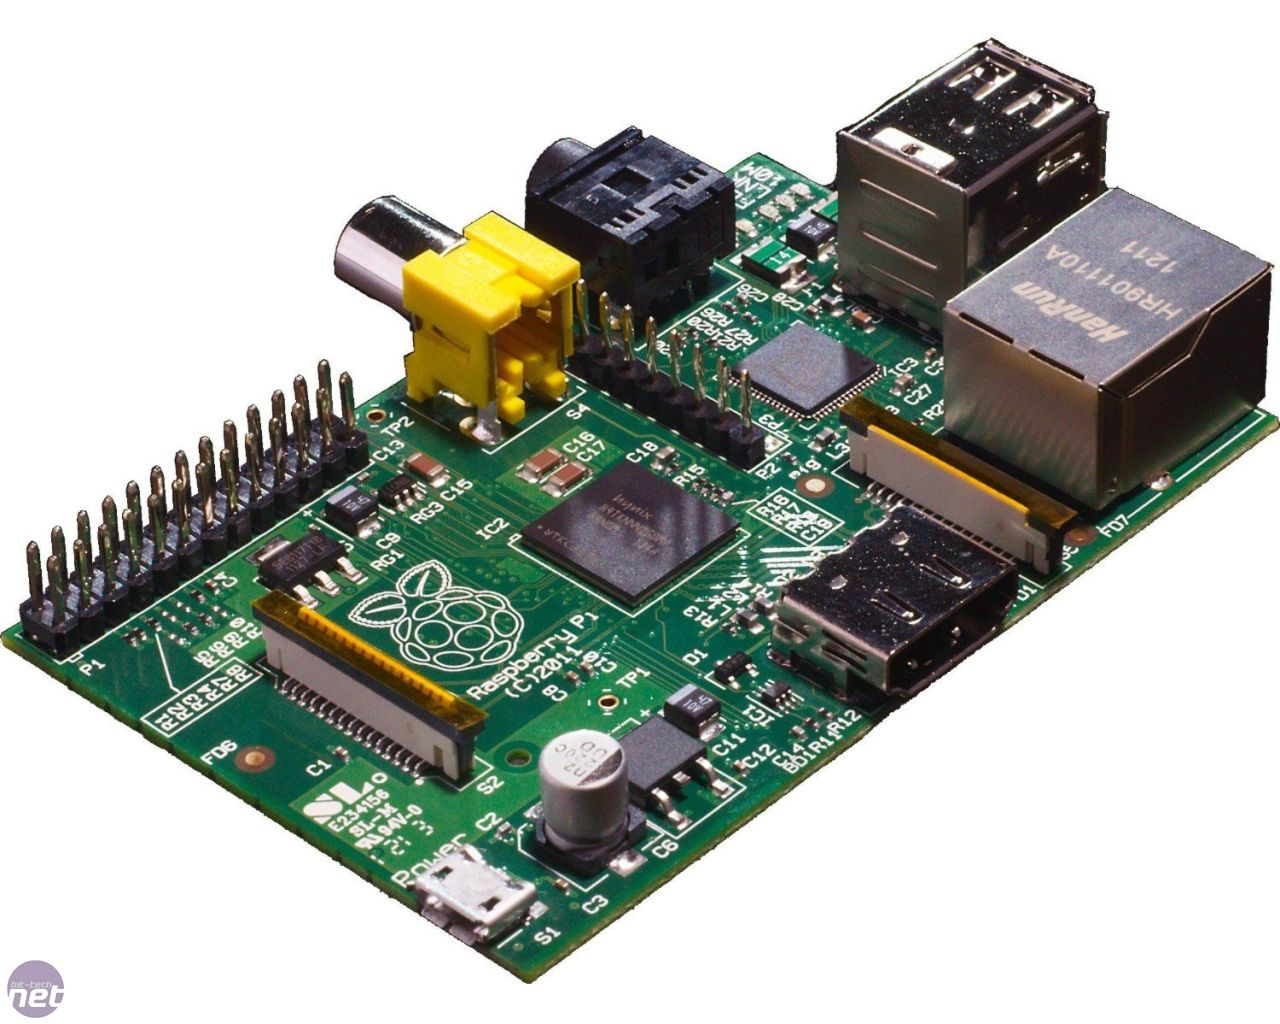
\includegraphics[width=4in]{rpi.jpg}
\caption{Raspberry Pi Rev. 2.}    
\end{figure}

\subsection{Changed Hardware}
The big change is the computer system. The old computer system is a Diamond Systems Athena II board that contains a VIA Mark Processor at 500MHz, 256MB RAM, running at a maximum of 8 watts, with 16 16-bit analog input analog-digital converters as well as 4 analog output 12-bit digital-analog converters. These are highly precise industrial strength ADC/DAC's that provide a very clean signal. We decided to replace this with a Raspberry Pi Rev. 2 shown in Fig 1. The Raspberry Pi is 700Mhz ARM11 processor, 512 MB ram, 2 easily accessible USB 2.0 ports, and uses a Secure Digital (SD) card for its storage. It has I$^2$C, SPI, UART, and a few GPIO ports. It has to be powered off a 5V line and requires a maximum of 700mA coming out to 3.5 watts. 

The Raspberry Pi requires a 5V power line, this is provided by a BEC that outputs a maximum of 3A. The new interface board has connections that allows easy replacement of this BEC with any other 5V voltage regular. The Raspberry Pi doesn't provide any analog-digital or digital to analog converters at all. We had to supplement this on the newer interface board. The Raspberry Pi's logic levels are also at 3.3V instead of 5Vs, therefore logic level converters have to be used to interface with the old interfaces. Sparkfun BOB-08745 bidirectional logic level converters are used as they allow the use on the bidirectional I$^2$C lines without confusing the Raspberry Pi's I$^2$C's bidirectional sensors. 

\begin{figure}
\centering
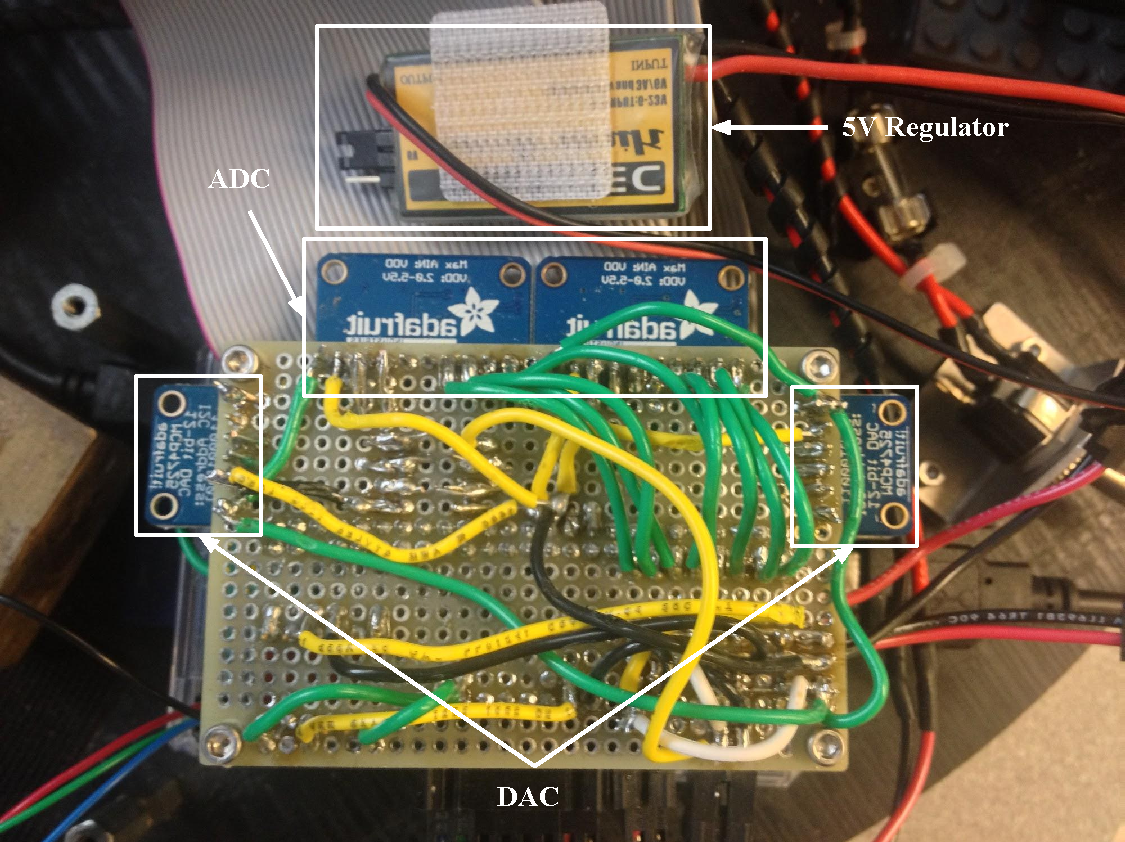
\includegraphics[width=7in]{interface_board_labels.pdf}
\caption{New interface board with ADCs, DACs, and 5V regulator.}    
\end{figure}

The analog-digital converters are ADS1115 16-Bit ADC with 4 channels. These ADCs allows four to be put on the same I$^2$C bus. We have 8 analog outputs from the various sensors, therefore we require two of these. We power this with 5V, and feed the 0-5V sensory directly in to the ADCS. The digital-analog converters are a MCP4725 Breakout Board which is a 12-Bit DAC that runs over I$^2$C. It also allows two of them to be on the same I$^2$C bus, which is perfect for us as we need exactly two DACs to send the signal to the fans. The old interface board requires a 0-10V analog signal, however the since the DACs that are compatible with the Raspberry Pi only output 0-5V analog signals, we add an op-amp that boosts that signal to 0-10V. Due to the the op-amp not being a rail-to-rail op-amp it requires a non 0V input for its absolute minimum or else the op-amp outputs the maximum voltage instead of the minimum. For our op-amp we need to output a minimum of 1V for the op-amp to recognize that it is actually receiving an input. Both ADC and DAC are hooked up to the Sparkfun logic level converter which lowers the 5V I$^2$C lines to the required 3.3V for the Raspberry Pi. Figure 2 shows a picture of the bottom of this interface board on top of the Raspberry Pi. Figure 3 shows a diagram of how the two interface boards are connected to each other.

\begin{figure}
\centering
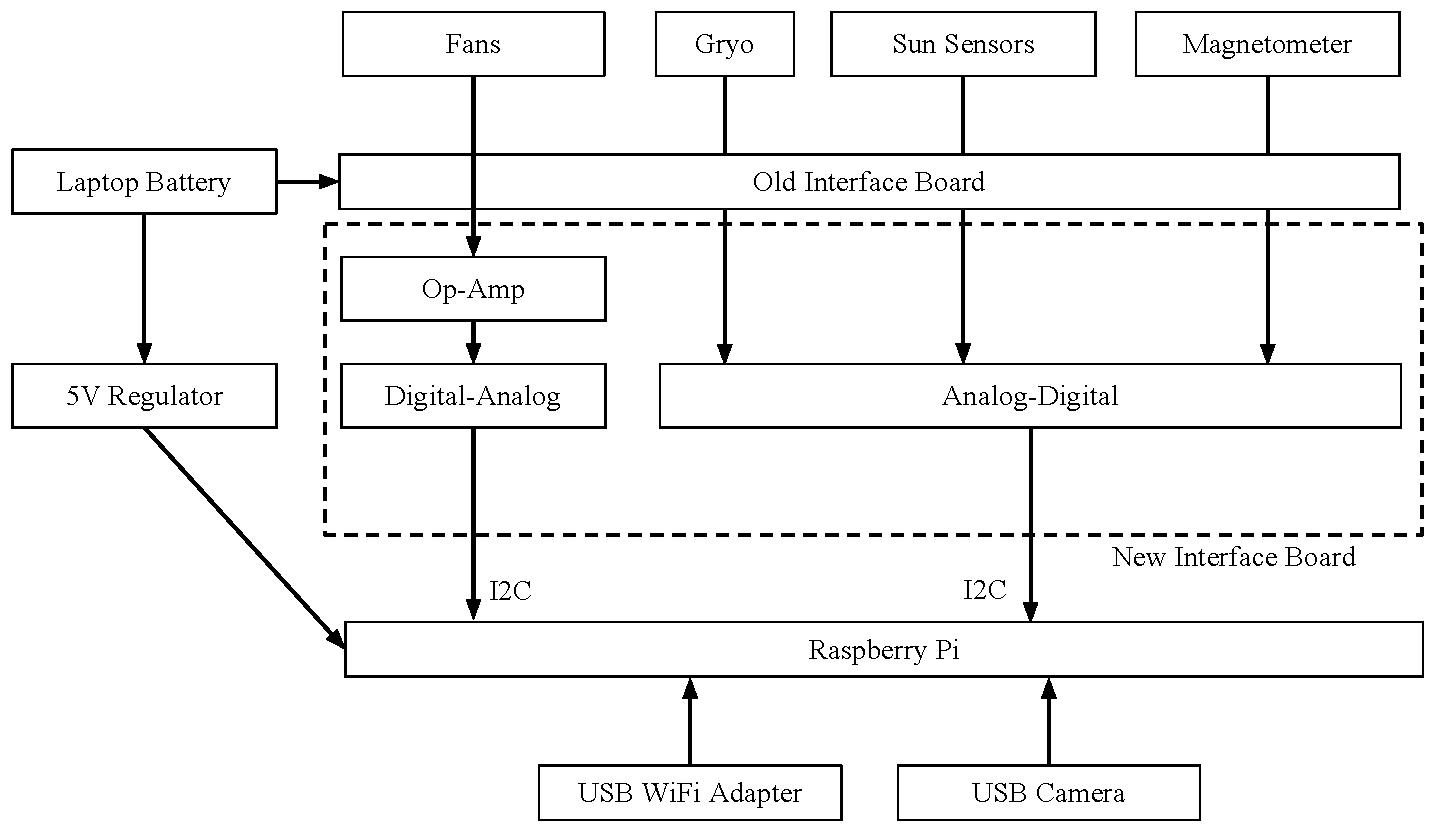
\includegraphics[width=6.5in]{Hardware_diagram.pdf}
\caption{Hardware diagram showing what is new and what is old.}
\end{figure}

The Monoprice Ultra-Mini USB Wireless Lan 802.11N Adapter is used to provide Wifi access to the Raspberry Pi fulfill the requirement of wireless turning. To add some computer vision component to the TableSat platform we also add a Point Grey FireFly FMVU-03MTC USB 2.0 camera. The Raspberry Pi doesn't have enough processing power to actually do any significant image processing. However it does have a GPU that allows for H.264 encoding. We'll utilize that GPU to provide a real time 30 frames per second streaming of 320x240 images system to allow another computer to do the vision processing.

\section{Software}
The software on the Raspberry Pi will obviously differ from the one on the Athena. The Athena runs on a QNX operating system while the Raspberry Pi runs on a custom version of the Debian operating system. The drivers that work for the Athena's ADCs and DACs do not work with the Raspberry Pi as the actually hardware is completely different. Linux offers tools to write to I$^2$C buses already in the kernel, therefore the basics of the Athena drivers are reproduced on the Raspberry Pi with its own drivers. This allows a very similar interface to both the ADC and the DAC without exposing the I$^2$C interface to the users.

The software for the camera requires the GPU library for hardware accelerated encoding. There are many limitations with the GPU library therefore the only encoding that was able to be done is from raw RGB to H.264 video format. The library isn't the most stable library so measures had to be done to make sure that the library will output encoded frames in real time as well as producing frames that could actually be decoded by the software decoder on the other end. The pipeline for the hardware encoding is detailed in Fig 4.

The process entails first getting the image from the camera, however the image from the camera are under a Bayer filter, therefore you have to remove that filter by Demosaicing. Since there are limitations of the GPU of the the Raspberry Pi we can't use the GPU to do the Demosaicing. This is the only reason why we are forced to run a cheap software Demosaicing that requires downsampling the image from 640x480 to 320x240 to keep real time as well as the 30 frames per second. After the software Demosaicing, we send the the image to the GPU input buffer. The GPU will encode this image and output a encoded frame. We empty this frame back into userspace memory, and check if this is a full frame. If it isn't a full frame we loop at grabbing frames while combining until we get a full frame. This is then end to the network, and the loop starts over. The one glitch in this entire pipeline is that the first frame that the GPU outputs just describes the coming H.264 stream, it doesn't contain any frames at all. This actually works out for the GPU, since the GPU requires a queued up frame before it finishes processing the current frame. What this means for the sequence of the images is that the computer receiving the images on the other end of the networking socket is always delayed by 1 frame, since that frame is stuck inside the GPU.

Over the network communication is handled over the User Datagram Protocol (UDP) by a library called UDT\footnote{http://udt.sourceforge.net/}. It is a library that handles communication over UDP. It overcomes one vital aspect of the UDP, which is UDP isn't reliable. UDP doesn't know or care about if the packets its sending are actually received. UDT actually incorporates a reliability factor to overcome this downside. Since we are streaming H.264 video stream instead of images by images to drastically reduce the bandwidth. Decoding a video stream requires every frame as each frame is dependent on the previous frames, therefore this reliability factor is extremely important. This library has also won many awards for its outstanding use of the full bandwidth of UDP.

We also set up a cross compiling system on an standard Ubuntu Linux system. This allows compilation of simple programs such as programs that use the I$^2$C libraries. There are significant advantages to have a cross compiler. The ability to compile on the Raspberry Pi is not taken away since certain programs such as the GPU encoding programs requires libraries that are extremely hard to reproduce in a cross compiling environment.

\begin{figure}
\centering
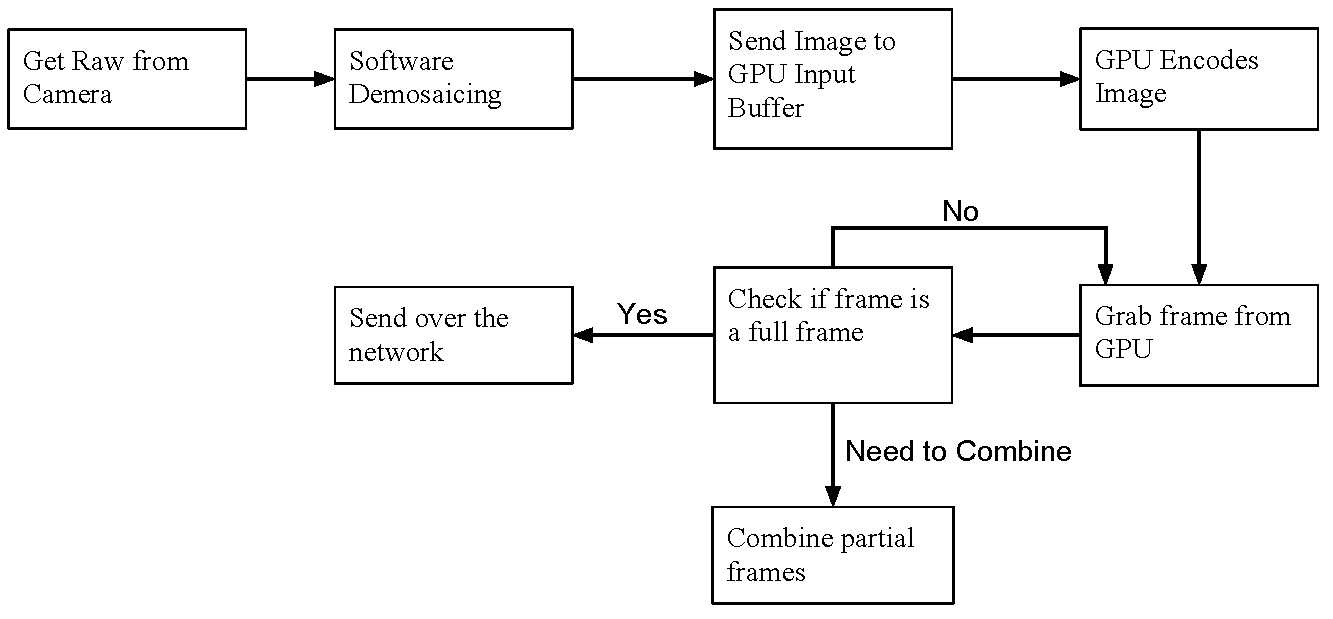
\includegraphics[width=6.5in]{GPU_encoding.pdf}
\caption{Hardware encoding pipeline}
\end{figure}

\section{Advantages of the Raspberry Pi}
There are many advantages to using the Raspberry Pi. First the old Athena system requires another QNX machine for compilation of code. This complicates the access to the actually TableSat system. To get code running on the TableSat, you must first write the code on your own computer, transfer to a computer in the lab, then transfer to another computer that runs QNX to compile for the TableSat system, and then transfer to the Raspberry Pi. This overall process also requires both the use of the SSH, SCP, TELNET, and FTP program. This is a significant disadvantage for the original system. The Raspberry Pi allows for either compilation on the actual Raspberry Pi or on a cross compiling system which is easily installed on a standard Linux system. This means the process has one less machine, which is the QNX compilation machine. The Raspberry Pi is accessible with SSH, and SCP, removing the need to learn how to use TELNET, and FTP to access and transfer files.

Another advantage of the Raspberry Pi is that it boots a version of Debian Linux instead of QNX. Many students are already familiar with Linux programs, however many of these programs are not available or behave in different ways. Debian Linux allow for easy development as well, since QNX isn't as popular and libraries might not be readily available, however most libraries can be compiled right on the Raspberry Pi system since it does support the Aptitude package manger. This might be significantly useful for the future to develop more applications for TableSat. An example of this is the application of computer vision that we have shown in this paper.

The Raspberry Pi also shows an advantage in the power required to run the system. The Athena board could use up to 8 watts of power while the Raspberry Pi will cap out at 3.5 watts and it often sits on at most 2 watts of power. This allows a longer up time for TableSat as there is quite a few periods of time where the fans are not running. The Raspberry Pi is also significantly cheaper and easily replaceable. This allows repairs to be done easily, and since the Raspberry Pi is so plug and play with the new interface board, it is as simple as putting in the old SD card into a new Raspberry Pi and reconnecting it.

\section{Experiments}
As found out by previous students, while the full PID controller can be utilized to control TableSat, a bang-bang controller does the job well enough to try and maintain a specific Gryo volts. The bang-bang controller here shows a P value of 1000, however there isn't much difference between different P values, and 1000 allows the reach from 0 to desired speed much faster and it doesn't change the oscillation since we can start spinning the other fan to force it back to the desire Gryo volts. Figure 5 shows a graph of trying to hit 4V on the Gryo. You can tell that 

\begin{figure}
\centering
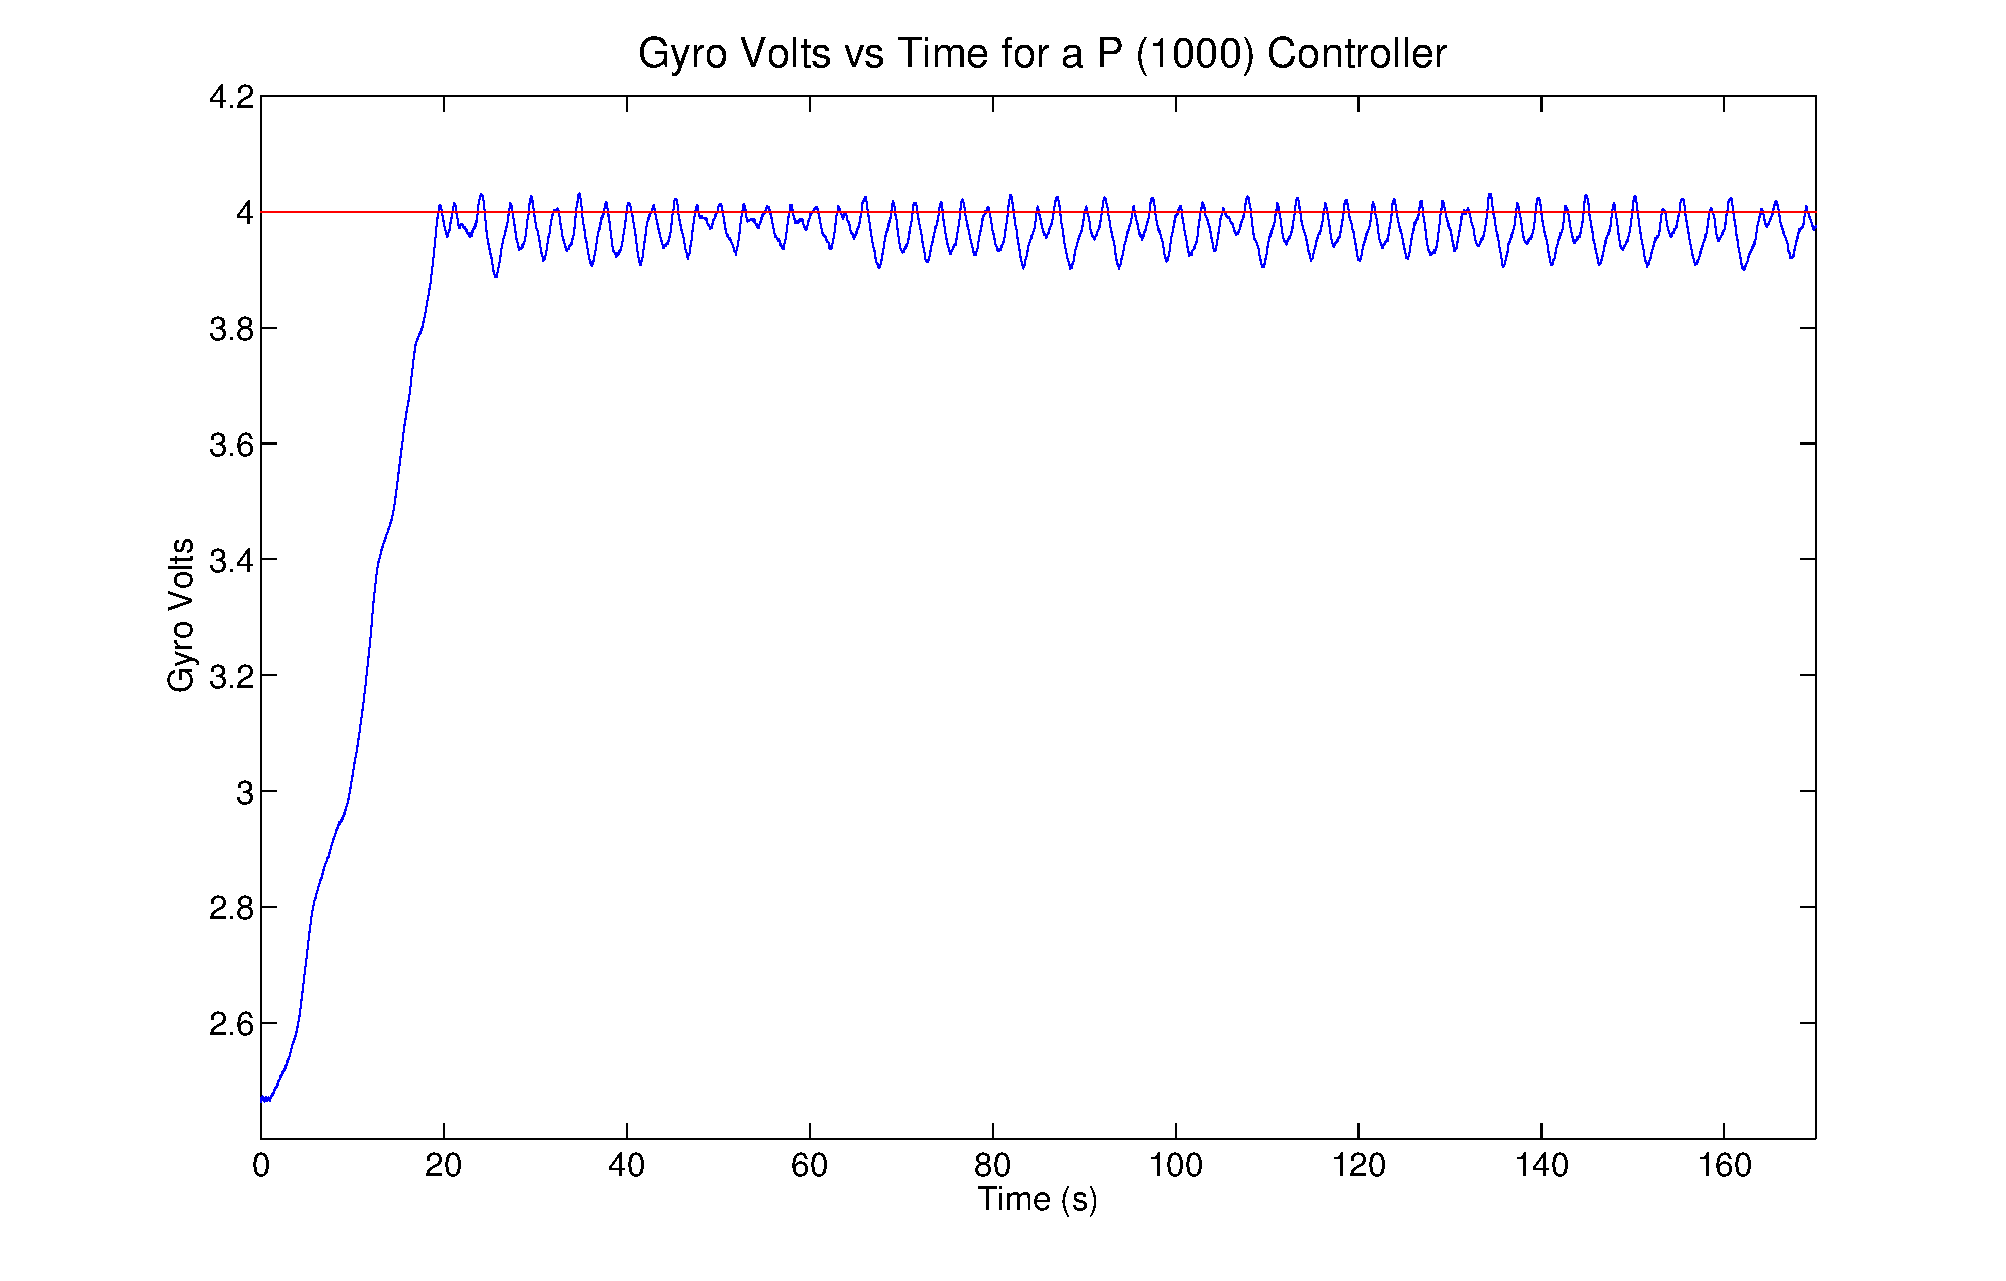
\includegraphics[width=\linewidth]{bang-bang.pdf}
\caption{PID bang-bang controller to 4 Gryo volts. Blue is measure from Gyro and Red is the setpoint. The X access is Time in seconds.}
\end{figure}

We also did an experiment to prove that the hardware encoding actually works. This experiment is, we got images from the camera and we streamed it to a ground station to do sparse optical flow and we averaged all the X velocities. Figure 6 shows the comparison of the two after normalization to normalize pixels to Gryo volts as best as possible. As you can see sparse optical flow seems to follow the trend, however at certain portion it spikes. These spikes can be attributed to certain features that were found for sparse optical flow wasn't good features to track and were apparent in the close space around the original feature causing a large change in position of the feature. We see that it follows the trend extremely well, the ramp up to the setpoint has some rough edges, but still seems acceptable. Towards the end of the run we tried to add interference by waving my hand around the cameras. This clearly causes extremely failure in the optical flow. Figure 7 shows a zoomed in version of this behavior. 

Figure 8 shows a zoomed in version of a period where the optical flow best matched the Gyro volts. As we can tell from this zoomed in version of the graph, we see that the optical flow can't capture the right magnitude of the movements. This graph is already normalized, and the optical flow seems to always be at around half of the the Gryo volts. This can be attributed to the fact that sometimes the features are stuck on a pixel and we don't have enough resolution to figure out that they've moved that far. Since with images features are not as invariant as we want, the algorithm will try to match as many of the features as possible however mismatches would greatly reduce the correctness of the optical flow algorithm. Overall this is a good proof that you can do off-board vision processing with the on-board hardware encoding and transmitting that video over the network to a dedicated vision processing computer.

\begin{figure}
\centering
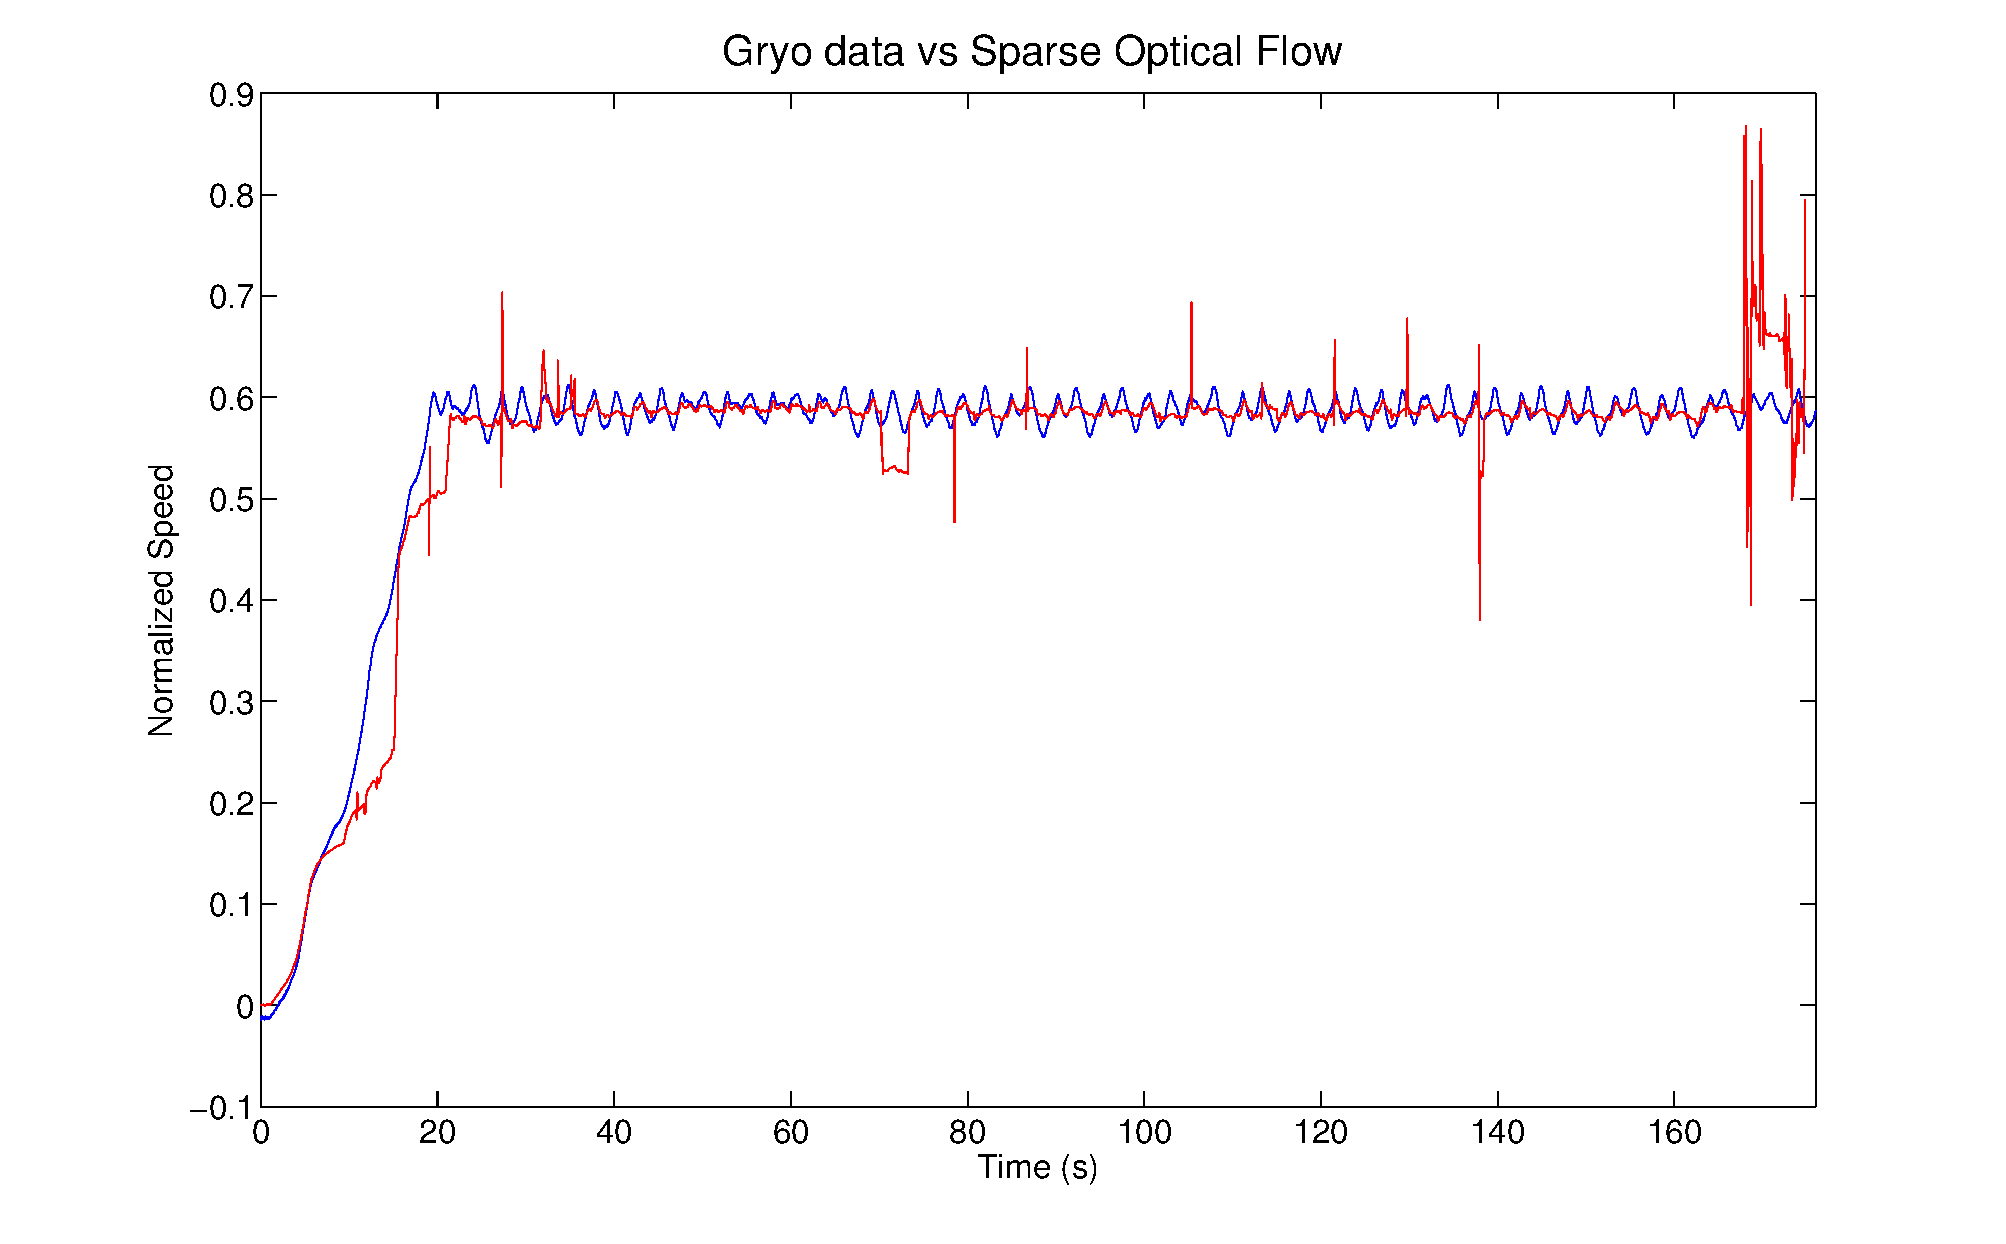
\includegraphics[height=4in]{fulltestcomp.pdf}
\caption{Comparison between the value measure by the Gyro and the value calculated by sparse optical flow. Blue is Gyro volts, Red is sparse optical flow.}
\end{figure}

\begin{figure}
\centering
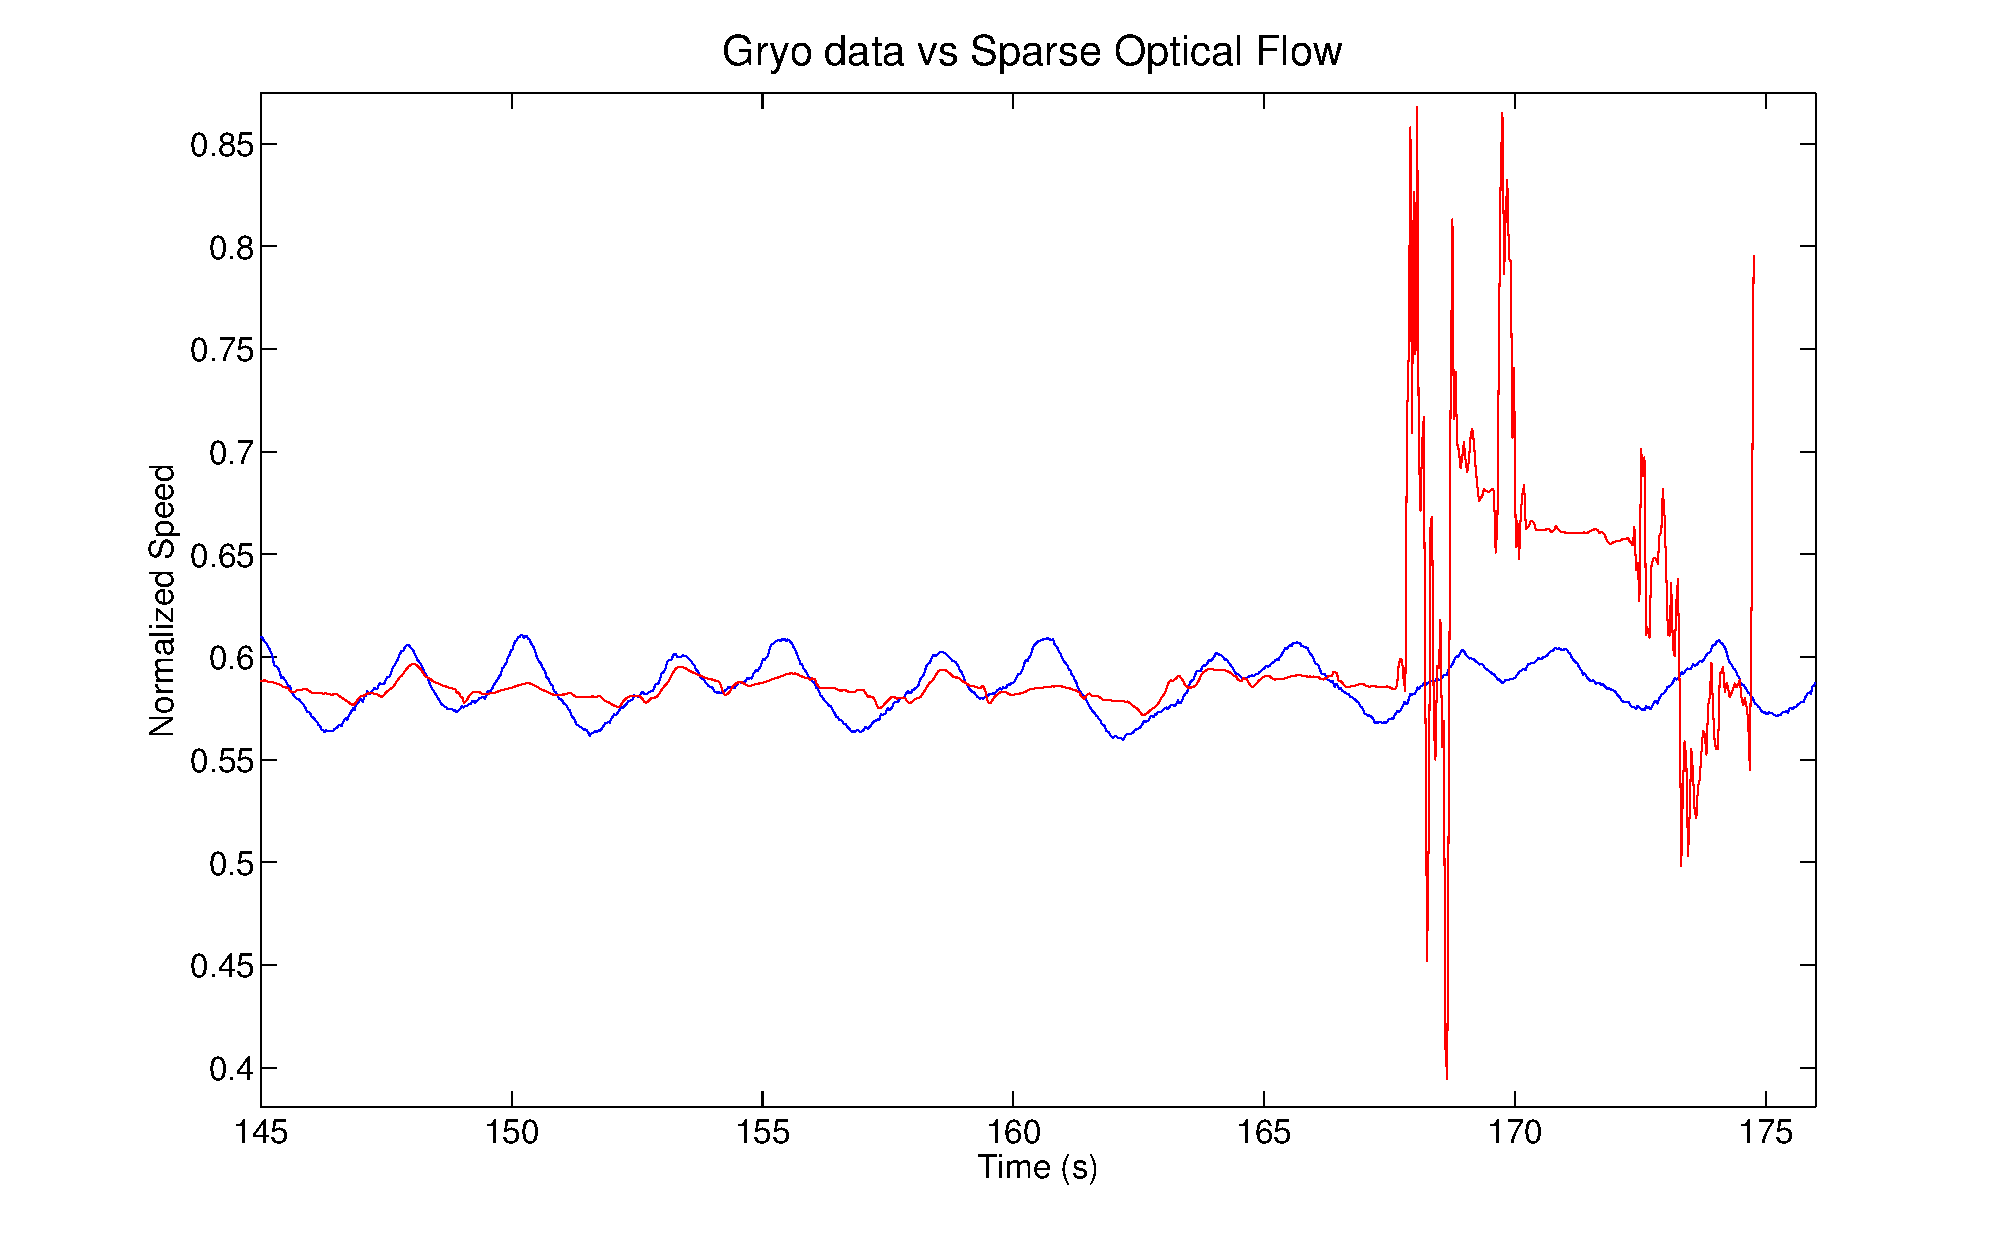
\includegraphics[height=4in]{badtestcomp.pdf}
\caption{Comparison between the value measure by the Gyro and the value calculated by sparse optical flow under extreme interference in the images. Blue is Gyro volts, Red is sparse optical flow.}
\end{figure}

\begin{figure}
\centering
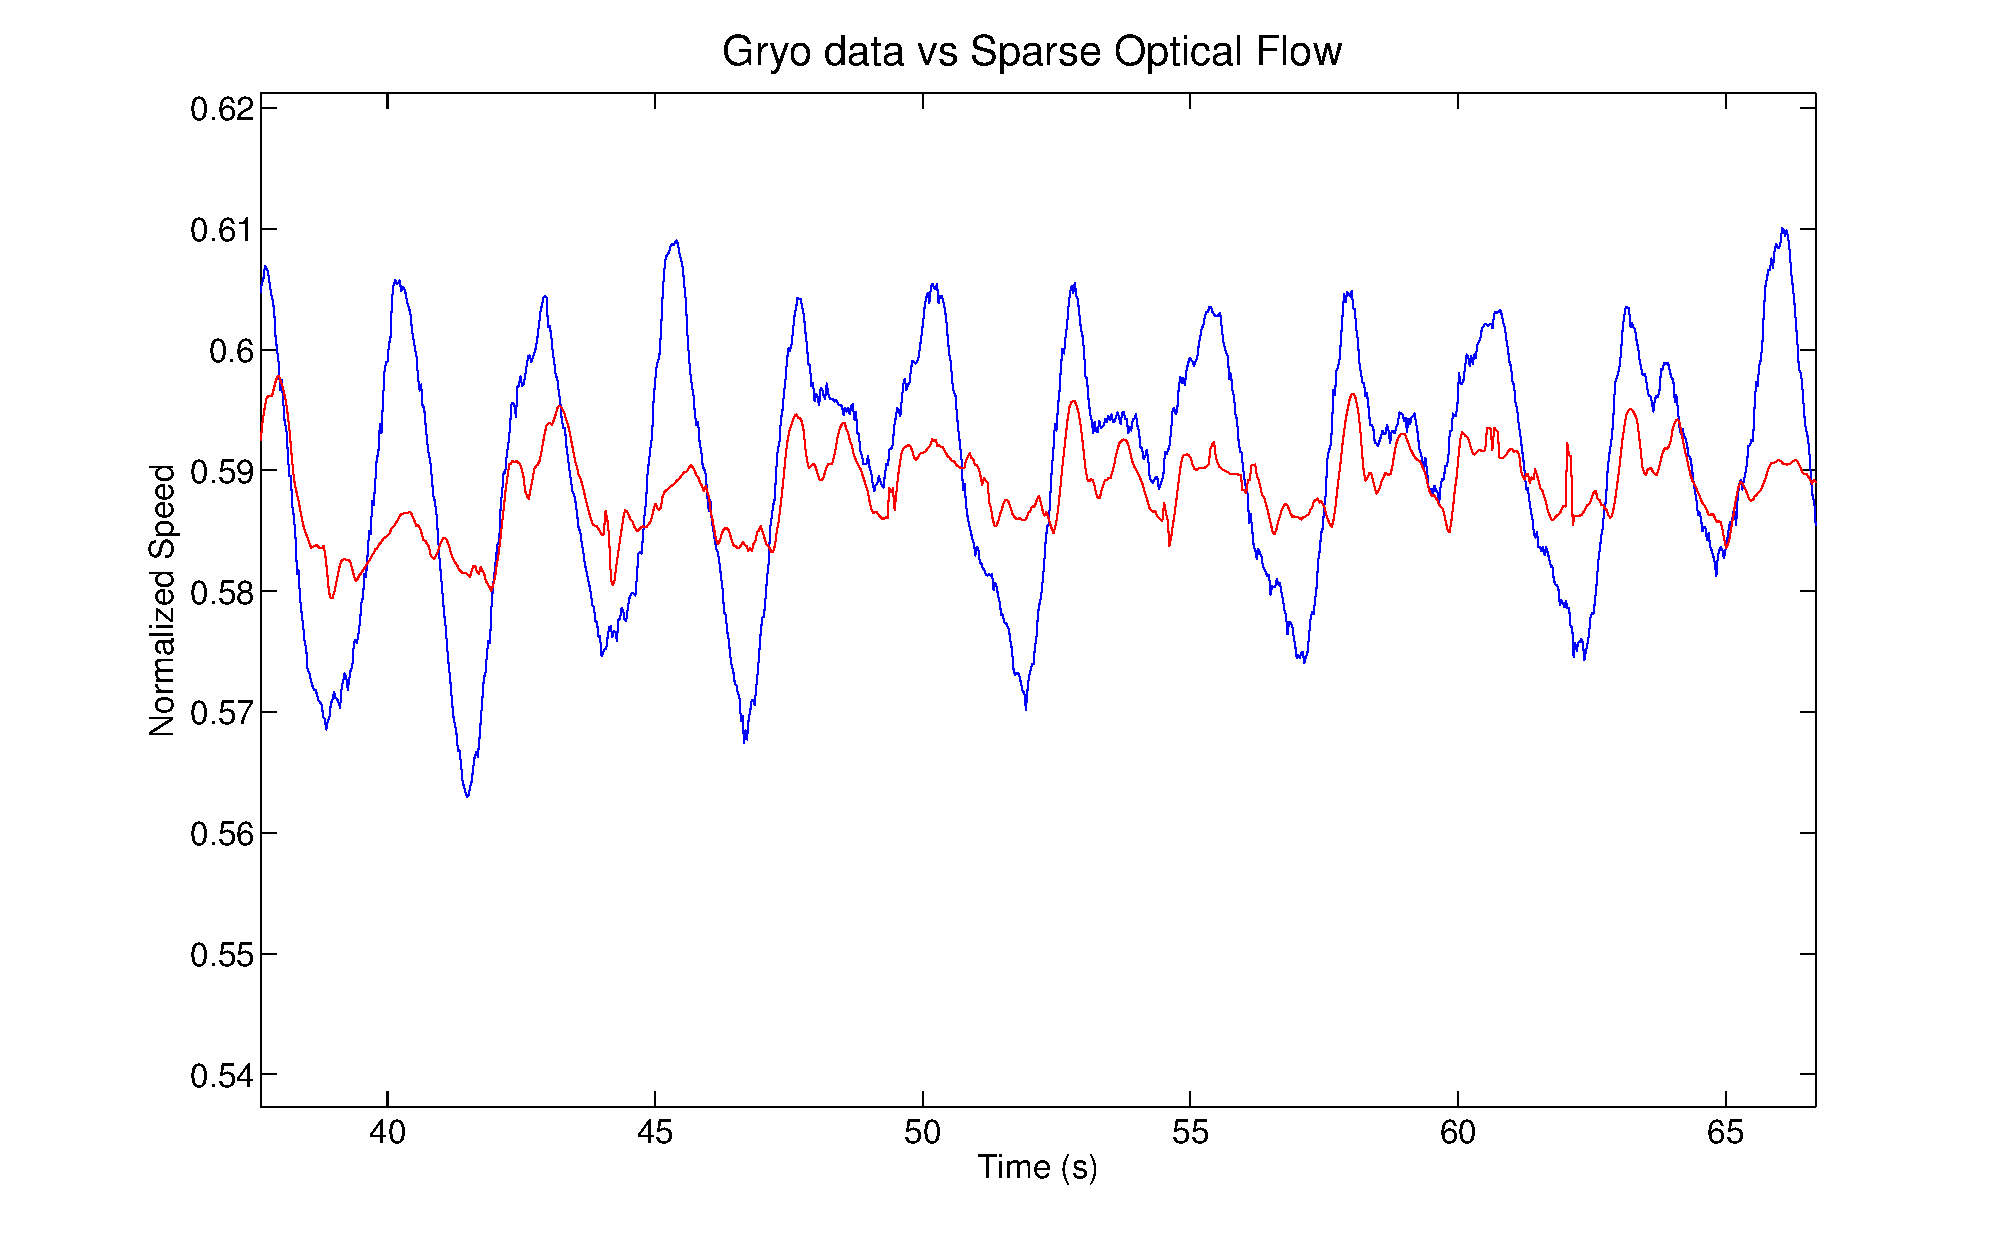
\includegraphics[height=4in]{goodtestcomp.pdf}
\caption{Comparison between the value measure by the Gyro and the value calculated by sparse optical flow where the two were best matched. Blue is Gyro volts, Red is sparse optical flow.}
\end{figure}

\section{Conclusion}
We have provide a much needed upgrade to TableSat to allow the overall platform higher accessibility and functionality. The use of a more standard Linux system and a cheaper, arguably more well known hardware platform allows students and future innovators to easily use and upgrade the system. We have shown that this new system is capable of performing the same tasks as before as well as showing that you can use the newly introduced image streaming to do many computer vision tasks that you might not have been able to do before. This new system should allow students to use the system more reliably and have less problems when dealing with the architecture of the overall TableSat platform.

\end{document}